\documentclass[a4paper]{article}

%%%%%%%%%%%%%%%%%%%%%%%%%%%%%%%%%%%%%%%%%%%%%%%%%%%%%%%%%%%%%%%%%%%%%%
% Imports.
%%%%%%%%%%%%%%%%%%%%%%%%%%%%%%%%%%%%%%%%%%%%%%%%%%%%%%%%%%%%%%%%%%%%%%

\usepackage{amsmath,amssymb,amsfonts}  % Typical maths resource packages
\usepackage{graphics}                  % Packages to allow inclusion of graphics
\DeclareGraphicsExtensions{.pdf,.png}
\usepackage{epstopdf}				   % Package to avoid errors on .eps to pdf conversions

\usepackage{fancyhdr}				   % Redesign the header and footer
\pagestyle{fancy}
\fancyfoot{}
\fancyhead{}
\fancyhead[OR]{\thepage}
\fancyhead[EL]{\thepage}


%\usepackage[T1]{fontenc}			   % Vectoriel fonts
\usepackage[french]{babel}			   % For french quotes
\usepackage{xcolor, url}			   % For links' colour

\usepackage{color}                     % For creating coloured text and background
\usepackage{hyperref}                  
\usepackage{textcomp}

\usepackage{xcolor}

% Listings settings.
\usepackage{courier}
\usepackage{caption}
\DeclareCaptionFont{white}{\color{white}}
\DeclareCaptionFormat{listing}{\colorbox[cmyk]{0.95, 0.95, 0.95,0.01}{\parbox{\textwidth}{\hspace{15pt}#1#2#3}}}
\captionsetup[lstlisting]{format=listing,labelfont=white,textfont=white, singlelinecheck=false, margin=0pt}

\usepackage{float}
\usepackage[hyperref,framed]{ntheorem} % For creating nice definition boxes
\usepackage[all]{hypcap}
\usepackage{framed}
\usepackage{pstricks}
\usepackage{listings}                  % For code listings
\usepackage{makeidx}                   % For generating index
\usepackage{enumitem}				   % http://ctan.org/pkg/enumitem
\usepackage[nohyperlinks]{acronym}
\usepackage{Msc}

\RequirePackage[left=2.4cm,right=2.4cm,bottom=2cm]{geometry} % Redefine the page margins
%\usepackage[hmargin=2.4cm]{geometry}

\renewcommand{\labelitemi}{$\bullet$}

\renewcommand\lstlistingname{Listing}
\renewcommand\lstlistlistingname{List of listings}

%%%%%%%%%%%%%%%%%%%%%%%%%%%%%%%%%%%%%%%%%%%%%%%%%%%%%%%%%%%%%%%%%%%%%%
%\parindent 1cm
%\parskip 0.2cm
%\topmargin 0cm
%\bottommargin 0cm
%\rightmargin 0cm
%\leftmargin 0cm
%\oddsidemargin 1cm
%\evensidemargin 0.5cm
%\textwidth 15cm
%\textheight 21cm
%\makeindex

%%%%%%%%%%%%%%%%%%%%%%%%%%%%%%%%%%%%%%%%%%%%%%%%%%%%%%%%%%%%%%%%%%%%%%
%\renewcommand{\familydefault}{\sfdefault}

%%%%%%%%%%%%%%%%%%%%%%%%%%%%%%%%%%%%%%%%%%%%%%%%%%%%%%%%%%%%%%%%%%%%%%
% where are figures
\graphicspath{
  {./}
  {figures/}
  }

%%%%%%%%%%%%%%%%%%%%%%%%%%%%%%%%%%%%%%%%%%%%%%%%%%%%%%%%%%%%%%%%%%%%%%
%hyperref settings
\hypersetup{pdfauthor=Thomas Rouvinez, 
            pdftitle=HL7 Exchange Module, 
            pdfsubject=YourBookSubjectHere,
            colorlinks=true,
            linkcolor=black}

%%%%%%%%%%%%%%%%%%%%%%%%%%%%%%%%%%%%%%%%%%%%%%%%%%%%%%%%%%%%%%%%%%%%%%
% redefine some colors
\definecolor{shadethmcolor}{rgb}{0.9412,.9412,1.0000} % 
\definecolor{shaderulecolor}{rgb}{0.1529,0.2510,0.5451} % RoyalBlue 
\definecolor{lightergray}{gray}{0.95}
\definecolor{palegreen}{rgb}{0.7148,0.9219,0.6797} %pale green

%%%%%%%%%%%%%%%%%%%%%%%%%%%%%%%%%%%%%%%%%%%%%%%%%%%%%%%%%%%%%%%%%%%%%%
% define the theorem environments
% 1. definition
\theoremstyle{break}
\shadecolor{shadethmcolor}
\def\theoremframecommand{% 
\psframebox[fillstyle=solid,fillcolor=shadethmcolor,linecolor=shaderulecolor]} 
\newshadedtheorem{definition}{Definition}[section]
% 2. remark
\theoremstyle{plain} 
\theoremheaderfont{\normalfont\footnotesize\bfseries} 
\theorembodyfont{\normalfont\footnotesize} 
\theoremsymbol{\ensuremath{\clubsuit}} 
\theoremseparator{.}
\theoremindent1cm 
\theoremprework{\smallskip} 
\theorempostwork{\smallskip} 
\newtheorem*{remark}{$\rightarrow$ Remark}
% 3. seobs (software engineering observation)
\theoremstyle{plain} 
\theoremheaderfont{\normalfont\bfseries}
\theorembodyfont{\normalfont\normalsize}  
\theoremsymbol{\ensuremath{\clubsuit}} 
\theoremindent0cm 
\theoremseparator{.} 
\theoremprework{\bigskip\hrule} 
\theorempostwork{\hrule\bigskip} 
\newtheorem{seobs}{Software Engineering Observation}[section]
% 4. program output
\theoremstyle{nonumberplain} 
\theoremindent0.5cm 
\theorembodyfont{\ttfamily\small}
\theoremindent0cm 
\theoremseparator{} 
\theoremprework{\bigskip\verb}
\theorempostwork{\bigskip} 
\shadecolor{shadethmcolor}
\def\theoremframecommand{% 
\psframebox[fillstyle=solid,fillcolor=palegreen,linecolor=palegreen]} 
\newshadedtheorem{programoutput}{}

%%%%%%%%%%%%%%%%%%%%%%%%%%%%%%%%%%%%%%%%%%%%%%%%%%%%%%%%%%%%%%%%%%%%%%
% settings for the listings

\definecolor{green}{RGB}{0,180,10}
\definecolor{dkgreen}{rgb}{0,0.6,0}
\definecolor{gray}{rgb}{0.5,0.5,0.5}
\definecolor{mauve}{rgb}{0.58,0,0.82}

\lstset{
		language=Java,                % the language of the code
  		basicstyle=\footnotesize\ttfamily, % Standardschrift
        numbers=left,               % Ort der Zeilennummern
        numberstyle=\tiny,          % Stil der Zeilennummern
        stepnumber=1,               % Abstand zwischen den Zeilennummern
        numbersep=8pt,              % Abstand der Nummern zum Text
        tabsize=2,                  % Groesse von Tabs
        extendedchars=true,         %
        breaklines=true,            % Zeilen werden Umgebrochen
        commentstyle=\color{dkgreen},
        keywordstyle=\color{mauve},
    	   frame=b,         
        stringstyle=\color{blue}\ttfamily, % Farbe der String
        showspaces=false,           % Leerzeichen anzeigen ?
        showtabs=false,             % Tabs anzeigen ?
        xleftmargin=17pt,
        framexleftmargin=17pt,
        framexrightmargin=5pt,
        framexbottommargin=4pt,
        %backgroundcolor=\color{lightgray},
        showstringspaces=false      % Leerzeichen in Strings anzeigen ?     
 }

\begin{document}
\pagenumbering{roman}

%%%%%%%%%%%%%%%%%%%%%%%%%%%%%%%%%%%%%%%%%%%%%%%%%%%%%%%%%%%%%%%%%%%%%%
% Custom commands.
%%%%%%%%%%%%%%%%%%%%%%%%%%%%%%%%%%%%%%%%%%%%%%%%%%%%%%%%%%%%%%%%%%%%%%

\newenvironment{listCustom}{
 \begin{list}{{$\bullet$}}{		% type of item representation
  \setlength{\partopsep}{0pt}
  \setlength{\parskip}{0pt}
  \setlength{\parsep}{0pt}
  \setlength{\topsep}{5mm}
  \setlength{\itemsep}{1mm}		% space between items
  \setlength{\labelsep}{0.25cm} % bullet to text distance
  \setlength{\leftmargin}{2cm}  % reset margin
 }
}{
 \end{list}
}

{\setlength{\leftmargini}{2cm} 
\newenvironment{listCustomNumber}{
 \begin{enumerate}{		% type of item representation
  \setlength{\leftmargin}{2cm}  % reset margin
 }
}{
 \end{enumerate}
}

\newcommand*{\xml}[1]{\texttt{<#1>}}

\newcommand*{\webquote}[1]{\textsf{\og #1 \fg{}}}
	
%%%%%%%%%%%%%%%%%%%%%%%%%%%%%%%%%%%%%%%%%%%%%%%%%%%%%%%%%%%%%%%%%%%%%%
% Title page.
%%%%%%%%%%%%%%%%%%%%%%%%%%%%%%%%%%%%%%%%%%%%%%%%%%%%%%%%%%%%%%%%%%%%%%

\title{User recognition on handwritten digits}
\course{Applied Signal Processing}

\author{Thomas Rouvinez, Didier Aeberhard}
\professor{Andreas Humm}
\date{May 16, 2014}


\rrno{}
\maketitle

\pagebreak


%%%%%%%%%%%%%%%%%%%%%%%%%%%%%%%%%%%%%%%%%%%%%%%%%%%%%%%%%%%%%%%%%%%%%%
% Content Table.
%%%%%%%%%%%%%%%%%%%%%%%%%%%%%%%%%%%%%%%%%%%%%%%%%%%%%%%%%%%%%%%%%%%%%%
	
\tableofcontents

\pagebreak

\pagenumbering{arabic}

%%%%%%%%%%%%%%%%%%%%%%%%%%%%%%%%%%%%%%%%%%%%%%%%%%%%%%%%%%%%%%%%%%%%%%
% Document.
%%%%%%%%%%%%%%%%%%%%%%%%%%%%%%%%%%%%%%%%%%%%%%%%%%%%%%%%%%%%%%%%%%%%%%

\section{Project description and goals}

During this project we intended to design and implement a system to match writing samples with their respective writers. To simplify the development, we will only focused on hand-written digits. We created our own database of samples to identify users. The goal of this project lies in being able to quickly identify a writer based on how he/she writes digits. We implemented the solution using Python(x,y) and the PIL library for image processing. In the following sections, we present the pipeline of the recognition process. Then each element is detailed separately from data acquisition and preprocessing, feature selection and extraction, classification and experiments.

\section{Program pipeline}

In this section we describe the pipeline of operations done throughout the whole process of user’s writing identification.\\

The first step consists in generating a feature vector for each user. For each user we captured a grid of hand-written digits and each sample is cut in a separate buffer. Cutting is done in two steps: first cell by cell, then we used an automatic crop function to isolate the digits. The features are then computed on each sample and regrouped per digit (mean values).  The extracted feature vector of each user it then used as input for the neural network that will be trained on the data. The results of the neural network is tightly related to the choice of features it uses as input. We could use a primary component analysis or search subsets to isolate information-worthy features, but we chose to leave that task to a genetic algorithm. The genetic algorithm will take care of selecting the best set of features to maximize the hit ratio of the neural network. Each feature will be considered as a gene and different combinations will lead to different results.\\

We chose to use neural networks because most of the processing time required goes into training. This implies that the execution time is more suited to real-time applications. To identify the user based on an input sample, the program has to extract the features out of the sample and run it through the best neural network selected by the genetic algorithm. The result will be a matching percentage for all the users. The highest percentage will most likely be the user who wrote the input sample.

\section{Data acquisition}

Recognition of users based on their writing requires initial data to extract user-dependant features from. Capture of this data is performed by asking different users to write down ten times each number from zero to nine in a grid. The grid is composed of one row per number type and ten columns to store ten variations of each number. By doing so we ensure that the features extraction will capture more details about the user’s writing techniques and style. Also multiple initial data will ease the feature extraction as the mean values across the ten variations will carry more meaning rather than using a single piece of data (only one digit image per number).\\

For this project, we created a table made of squares to host the writing of the users. Each square is 300 pixels wide bounding box. This was done to ensure the users do write in a defined space to ease the samples’ extraction. Figure 1 illustrates the capture of ten variations of the zero digit from a single user.

\vspace{1mm}
\begin{figure}[h!]
  \caption{User grid with number from 0 to 2.}
  \centering
    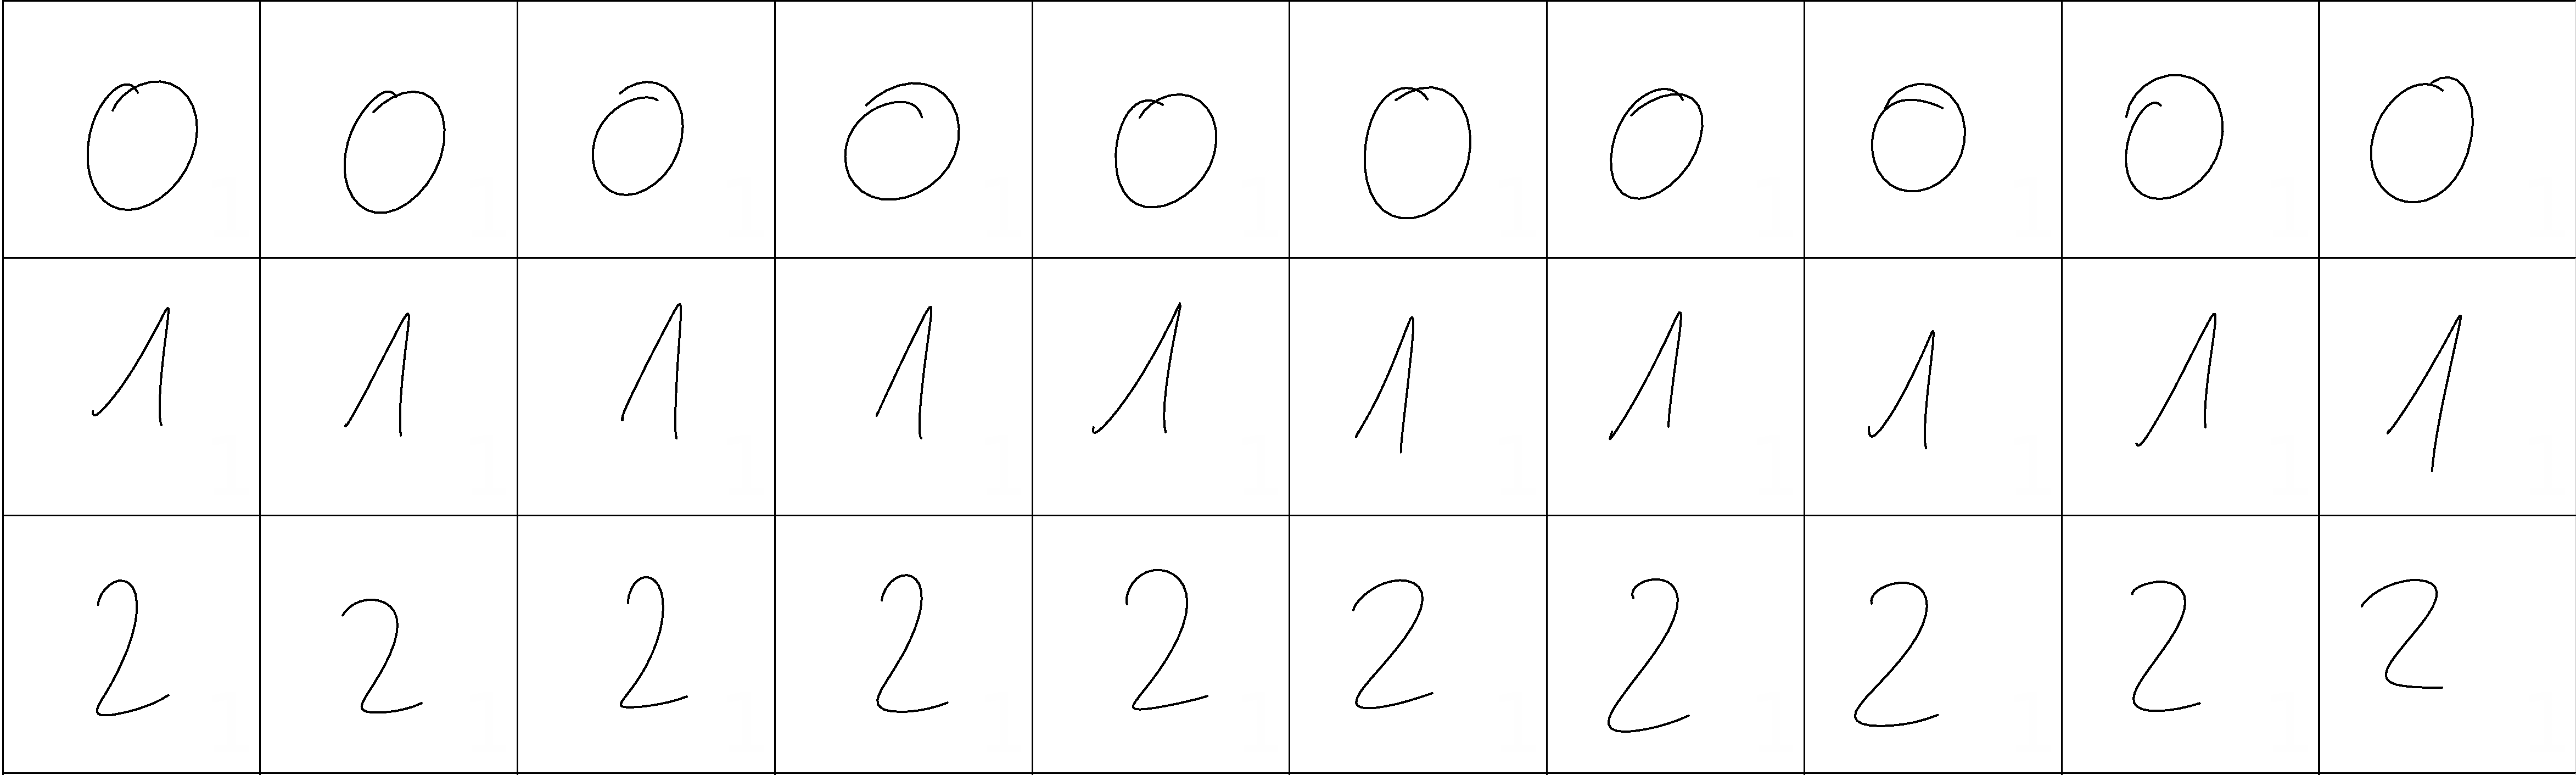
\includegraphics[scale=0.095]{didierNumbers}
\end{figure}

We use offline data as it most often depicts better the real problem to solve in user recognition based on user handwriting. Such data is also harder to recognize than the online data that contains additional information on writing speed and character construction patterns. Not every user starts writing letters by applying the same stroke first. Offline data does contain much information that can be turned into features, but their extraction is harder to perform: the quality of the acquired samples may vary.\\

In order to avoid capture hazards and variations that may occur by using different types of paper sheets, different pens thicknesses and colors as well as scanning variations in quality (contrast and luminosity mostly as they can reveal or hide details), we decided to use a numerical acquisition system. We used an HP Compaq TC4200 tablet PC and asked the users to use the stylus to perform writings in the bounding boxes provided by the template grid prepared for data acquisition. This system does not influence the user’s writing and spares extensive pre-processing of the data.\\

During the capture process, we asked all users not to write down the ten variations of a single digit at once. By allowing the users to write for example all the zeros before proceeding further on we let them become subject to involuntary repetition of features. Upon repeated writing of the same character, the human mind progressively attributes less attention to the task and this leads to a “mindless” copy of the previously done action. This contradicts our will to capture multiple variations as the results will not end up being ten variations, but maybe only two or three real variations. To counter this we required that each user fills randomly the rows or moves in diagonal only in the data grid. This resulted is a better data acquisition from a qualitative point of view as each user had to think and focus on writing another type of digit each time. We performed this process on five different users and gathered the grids of digits. On the ten variations captured per digit, we will use six for the training set, two for the test set and two also for the validation set. The next section describes the pre-processing done on this data.

\section{Data pre-processing}

Data acquisition was performed digitally and thus most of the conventional pre-processing is unnecessary. In conventional cases a picture of the writing should be acquired via a scanner or camera. Then the image is converted into levels of grey to enhance contour detection and remove color variations that do not yield more useful information for features extraction. Then a combined filter of contrast and luminosity is applied to remove any glitches the digitalization process might have induced (paper quality, stains, etc). By capturing data with a tablet PC, we make sure there are only two colors (black and white) and no glitches nor noise.\\

Another set of pre-processing methods is skew and slant correction. Skew and slant represent the inclinations or the writing both horizontally considering the whole word or vertically considering each single character. In our case, skew and slant contain additional information that can translate into exploitable features for the classifiers. If skew may not bring much information, slant on the other hand can provide an information on the writing speed as people tend to write more vertically the slower they write. This provides us with an online-like feature extracted from an offline sample.

\section{Features selection and extraction}
\subsection{Statistical features}

Statistical features are quickly computed and extract a set of features that provide global information on the samples. They can be used in combination with other types of features to assess them. Statistical features are also cheaper processing-wise.

\subsubsection{Presence}
Presence takes all the pixels and computes the percentage of black pixels compared to the surface of the sample. Despite not being the most interesting feature, it provides an idea on how much space is used by the digit in the cell. For instance if a writer is used to use curves for the lower stroke of a 2, it will increase the presence compared to another writer who uses a straight line.

\subsubsection{Mean height and width}
For each user, we compute the mean height and width per digit. We achieve this by first extracting each cell from the grid, then use PIL’s\footnote{See \url{http://www.pythonware.com/products/pil/}} automatic crop function to isolate only the digit. Though simple, these two features already provide an information on the average size of the handwriting. Combining this information with other features scale dependent can yield interesting points to differentiate users.

\subsubsection{Center of gravity}
The center of gravity is computed by weighting the amount of black per row for the height and per column for the width. Doing so provides us with a tuple (x, y) that represent the coordinates of the center of gravity in the letter. For convenience, it is computed at the same time as presence since both features require to know the number of black pixels in the sample. The center of gravity provides information on the repartition in space of a digit.

\subsection{Structural}

Structural features require an in-depth analysis of the written digit but yield valuable information. We are more specifically interested in learning characteristics on the writing habits of the user such as the inclination of the digits (vertically and horizontally) or the inclination of strokes and their convergence/divergence. To achieve this, we proceed by clustering the samples dynamically using horizontal and vertical splitting.

\subsubsection{Horizontal splitting}

Horizontal splitting is a known process to extract a definite amount of points in offline signatures validation. The process is the following : 

\vspace{2mm}
\begin{enumerate}
	\item Split the sample horizontally in the middle, and extract for each half the center of gravity h0 and h1 based on the amount of writing in those areas.
	\item From h0 and h1, split vertically each horizontal half in order to get four distinct clusters in the sample.
	\item For each cluster compute the centers of gravity h2, h3, h4 h5.
\end{enumerate}
\vspace{2mm}

Once this process is done, we have extracted six points h0, …, h5. By tracing vectors going through different combinations of these points, we extract the main features. At the end of the splitting process, we can rebuild the strokes used to draw the digit. Indeed, by tracing lines between the six points in clockwise order we can get the main strokes required to draw the digit. The order would be v2, v3, v1,v0, v4 and v5. For this project recognizing the digits is not our focus. Hence we do not recreate the tracing, but analyse the differences of angles between the major strokes. This is done with the following features:

\vspace{2mm}
\begin{listCustom}
	\item H1: angle difference between (h0,h1) and (h2,h3). With these two lines we can extract the angle difference between the mid strokes and the upper ones. With digits like 1a,  2s, 7s or 9s this difference can vary a lot from one user to the other.
	\item H2: angle difference between (h0,h1) and (h4,h5). This is the opposite of H1 as we compare the mid strokes with the lower ones.
	\item H3: angle difference between (h2,h3) and (h4,h5). It compares the angle difference between the upper strokes and the lower ones. By leaving out the mid strokes, we compute a new feature that that depicts if the user is “opening” or “closing“ his digit. By opening we mean that h3 is higher than h2 and h5 lower than h4, making the two vectors opening the area between them as we move from left to right of the sample. A “closing” digit is the opposite.
	\item H4: angle difference between (h2,h3) and an horizontal line. Since we are performing the first cut horizontally, it can become interesting to compare the upper strokes with the horizon. It yields a more neutral feature than a direct comparison between two types of strokes (upper, mid, lower).
	\item H5: angle difference between (h4,h5) and an horizontal line. Same as H4 but with the lower strokes.
	\item H6: h0 and h1 alignment. This provides a simple information on the angle of the vector that describes the mid strokes.
	\item H7: h2 and h3 alignment. This provides a simple information on the angle of the vector that describes the upper strokes.
	\item H8: h4 and h5 alignment. This provides a simple information on the angle of the vector that describes the upper strokes.
\end{listCustom}
\vspace{2mm}

\vspace{1mm}
\begin{figure}[h!]
  \caption{Horizontal cut for the digit 2, with H6, H7 and H8 dawn.}
  \centering
    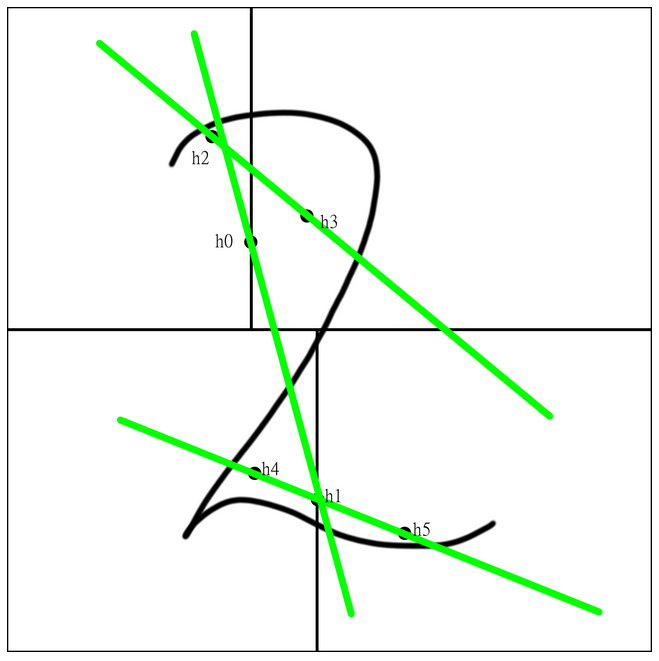
\includegraphics[scale=0.5]{hcut}
\end{figure}

Horizontal splitting provides multiple types of information that help determining the structural differences of the writing between two users. We also use the 6 points h0 to h5 as a feature. It depicts all the six centers of gravity in the sample and are very handwriting specific. With such features we can also approximate the skew of the writing.

\subsubsection{Vertical splitting}

Vertical splitting follows the same principle as horizontal splitting but we use the notation v instead of h to differentiate both types of splits. The main difference lies in the fact that the first cut is done vertically. This yields a different clusterization of the sample and thus new features. We use the same comparisons of vectors as in the horizontal split:

\vspace{2mm}
\begin{listCustom}
	\item V1: angle difference between (v0,v1) and (v2,v3). With a vertical split first, this feature tend to provide an inverse vector compared to H1. With digits such as 8s it represents better the skew as it cuts the digit vertically in two and then V1 cuts it in an horizontal fashion, giving an approximation of the inclination of the digit. 
	\item V2: angle difference between (v0,v1) and (v4,v5).
	\item V3: angle difference between (v2,v3) and (v4,v5).  With a different original split, the centers of gravity of each cluster changes and compared to H3, V3 shows the “opening” or “closing” more on the sides of the digit (if both vectors are more or less parallel).
	\item V4: angle difference between (v2,v3) and a vertical line. This feature yields a normalization of the magnitude of the first stroke.
V5: angle difference between (v4,v5) and a vertical line. Same as V4, but for the lower strokes.
	\item V6: v0 and v1 alignment. Depicts the diagonal cut of the digit.
	\item V7: h2 and h3 alignment. 
	\item V8: v4 and v5 alignment.
\end{listCustom}
\vspace{1mm}

\begin{figure}[h!]
  \caption{Vertical cut for the digit 2, with V6, V7 and V8 dawn.}
  \centering
    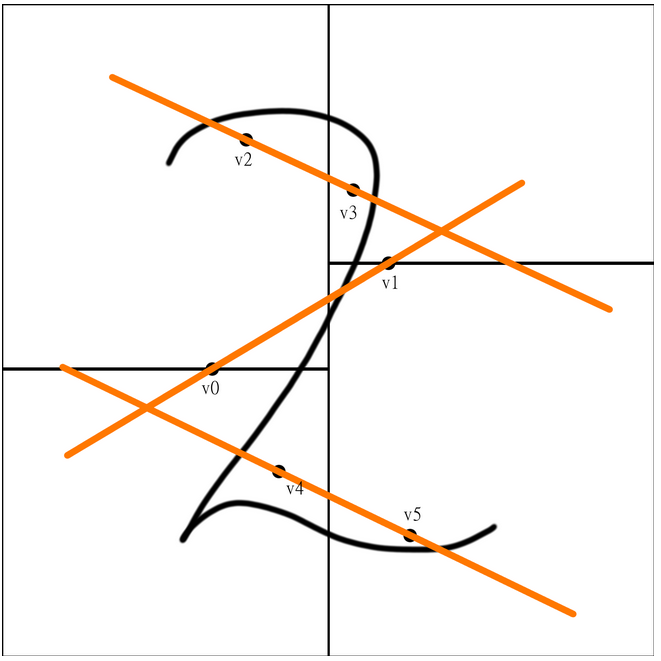
\includegraphics[scale=0.49]{vcut}
\end{figure}

Globally the H features provide more information on the direction of the digit and its orientation whereas the V features represent more the speed, magnitude and order of the movements of the writer.

\subsubsection{Combined splitting}

Having the six centers of gravity being computed for both horizontal and vertical splits, we chose to reuse this information and gather knowledge about the differences of each type of splits. Many possibilities of comparison are possible, for example in each type of cuts we could have tried to draw lines between (v2,v4) and (v3,v5) to approximate the slant of the writing. We chose not to do so because such information may vary much between two different variations of a digit. Therefore we added the following combined features:

\begin{listCustom}
	\item C1: angle difference between (h0,h1) and (v0,v1).
	\item C2: angle difference between (h2,h3) and (v2,v3).
	\item C3: angle difference between (h4,h5) and (v4,v5).
\end{listCustom}

As seen on figures 2 and 3, the two types of cuts generate very different distributions of the centers of gravity and comparing them can provide precious knowledge about the writing independently from scale or variations. Note that this process could be applied further on to gain a deeper knowledge on inflection points in the writing, but for the purposes of this project and because of the size of the samples we have, we decided not to go beyond four clusters.

\section{Classifying data}
\subsection{LSTM Recurrent Neural Networks}

Once the features’ extraction is done for each digits’ variation of each user, we store them into a “Users” data object. It holds an array of “User” objects. The User object stores the name, user-specific key\footnote{The user key is used as target output for the neural network. We then link the output of the neural network to the closest match.} and the features vectors for each digits. With this data we can now proceed to attempt to classify the data in order to recognize the users.\\

We chose to use PyBrain’s\footnote{See : \url{http://pybrain.org/}} neural networks library for python. It offers a wide range of neural networks including recurrent neural networks with long-short term memory. Neural networks need to be trained on the data before they are capable of classifying any data. This process takes time but allows instant execution once the training is done. We train one neural network per type of digit. Each neural network receives seven variations from each user. Each variation is made of 24 features that are input in the neural network. We use a Long-Short Term Memory hidden layer of 40 neurons and a single output neuron.  The networks are then trained with a back-propagation trainer and serialized for later usage. We also serialize the Users object as it represents the database of samples.

\section{Software manual}

In order to run this software, the following requirements should be met: first we use many libraries featured in the python(x,y) distribution\footnote{See \url{https://code.google.com/p/pythonxy/}} such as scypy and numpy. PIL is integrated in python(x,y) and does not need extra installation. However the PyBrain\footnote{Download and installation documentation: \url{http://pybrain.org/pages/download}} library should be installed separately. Once these prerequisites are installed, the software can be launched. For this purpose we use windows powershell, but any shell supporting the execution of python programs works. To launch the program, execute the following command in a shell:

\vspace{2mm}
\begin{lstlisting}
python .\extractor.py
\end{lstlisting}
\vspace{2mm}

Upon launch, the program will propose either to retrain the neural networks or to query them. By inputting "y" the program will take all the users as described in "extractor.py", compute the features and train all ten neural networks. Note that once this process is done the program will have to be restarted to perform any queries on the database. By inputting "n", the program will open a database-like query system. Each query requires the user to select a sample from the database. To do so, three arguments are asked: the digit to select, from which user (all users are found in ".\textbackslash Users\textbackslash username") and finally which variation of that digit should be selected. This sample is then input into the corresponding neural network and the output is returned. When possible, the output is matched with the best match known in the database. In figure \ref{guide1} we see that the user recognized is the user requested. The confidence level is also displayed and represents the difference in percentage between the output of the neural network and the rounded value of this output. Since we use integer keys for the users, by subtracting the key to the result of the neural network we obtain the "distance" between the user recognized and the actual user.

\begin{figure}[h!]
  \caption{Example of a query.}
  \centering
    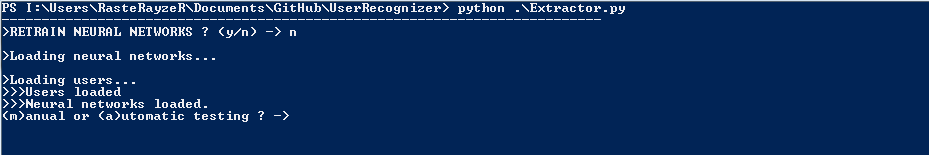
\includegraphics[scale=0.5]{guide1}
  \label{guide1}
\end{figure}

Once a query is performed, the program offers the possibility to perform another query. Note that these queries are linked together as they contribute to the recognition of the same user. If a single input is not enough to recognize the right user, then using other digits or variations of the same digit can help reducing the recognition error rate. Each subsequent query will be stored in the array of factors and a mean value is computed out of it. The mean value is then compared to the database of users. With more inputs, the confidence level or the recognition will also increase. In the next section, we present our results with a database of five users.

\section{Experimentations}

\section{Improvements}

%% Add GUI
%% Improve settings of the LSTM
%% Deeper analysis of what the features could bring, how to combine them

\section{Conclusions}

%%%%%%%%%%%%%%%%%%%%%%%%%%%%%%%%%%%%%%%%%%%%%%%%%%%%%%%%%%%%%%%%%%%%%%
% End of document.
%%%%%%%%%%%%%%%%%%%%%%%%%%%%%%%%%%%%%%%%%%%%%%%%%%%%%%%%%%%%%%%%%%%%%%

\end{document}